%%%%%%%%%%%%%%%%%%%%%%%%%%%%%%%%%%%%%%%%%
% FRI Data Science_report LaTeX Template
% Version 1.0 (28/1/2020)
% 
% Jure Demšar (jure.demsar@fri.uni-lj.si)
%
% Based on MicromouseSymp article template by:
% Mathias Legrand (legrand.mathias@gmail.com) 
% With extensive modifications by:
% Antonio Valente (antonio.luis.valente@gmail.com)
%
% License:
% CC BY-NC-SA 3.0 (http://creativecommons.org/licenses/by-nc-sa/3.0/)
%
%%%%%%%%%%%%%%%%%%%%%%%%%%%%%%%%%%%%%%%%%


%----------------------------------------------------------------------------------------
%	PACKAGES AND OTHER DOCUMENT CONFIGURATIONS
%----------------------------------------------------------------------------------------
\documentclass[fleqn,moreauthors,10pt]{ds_report}
\usepackage[english]{babel}
\usepackage[toc,page]{appendix}

\graphicspath{{fig/}}




%----------------------------------------------------------------------------------------
%	ARTICLE INFORMATION
%----------------------------------------------------------------------------------------

% Header
\JournalInfo{FRI Natural language processing course 2024}

% Interim or final report
\Archive{Project report} 
%\Archive{Final report} 

% Article title
\PaperTitle{Conversations with Characters in Stories for Literacy}

% Authors (student competitors) and their info
\Authors{Žan Kogovšek, Žiga Drab, Vid Cesar}

% Advisors
\affiliation{\textit{Advisors: Slavko Žitnik}}

% Keywords
\Keywords{Literacy Improvement, Dialogue Agents, Harry Potter, Pre-trained Large Language Models, RAG}
\newcommand{\keywordname}{Keywords}


%----------------------------------------------------------------------------------------
%	ABSTRACT
%----------------------------------------------------------------------------------------
% Abstract
\Abstract{
This paper explores using chatbots, particularly those modeled after literary characters, to boost children's literacy by making reading more engaging. We propose a pipeline for creating these character-driven chatbots and evaluate their effectiveness using large language models and retrieval augmented generation. Our results show significant improvements in question-answering abilities, especially when incorporating context from characters' stories. However, challenges remain, such as resilience to misinformation and language limitations. Future work should focus on fine-tuning models on characters' original stories to enhance performance and multilingual responses.
}

%----------------------------------------------------------------------------------------

\begin{document}

% Makes all text pages the same height
\flushbottom 

% Print the title and abstract box
\maketitle 

% Removes page numbering from the first page
% \thispagestyle{empty} 
%----------------------------------------------------------------------------------------
%	ARTICLE CONTENTS
%----------------------------------------------------------------------------------------

\section*{Introduction}

The declining interest in reading among young people and their challenges with advanced literacy skills pose significant risks to their academic and professional futures \cite{murray2021literacy}. To address this, innovative approaches are needed to reengage youth with literature.

Chatbots represent a promising solution. Research by Brandtzaeg et al. \cite{why_chatbots} shows their primary appeal lies in their entertainment value, suggesting chatbots could be used not only for information retrieval but also as engaging entertainment platforms.

Recent advancements in open-domain conversation models, such as those by Adiwardana et al. \cite{adiwardana2020towards}, have shown potential for chatbots to engage in more human-like conversations by incorporating real-life interaction traits like emotion \cite{zhou2018emotional} and empathy \cite{rashkin2018towards_empathy}. Zhang et al. \cite{zhang2018personalizing} further the development by enabling chatbots to generate responses that reflect consistent personalities, enhancing both personalization and engagement.

In this paper, we investigate how chatbots, modeled after literary characters, can boost children's literacy by making reading more interactive and appealing. We aim to develop a pipeline to create character-driven chatbots.

\section*{Related Work}

\subsection*{Articles}
Nielen et al. \cite{nielen2018digital} have explored enhancing children's literacy using technology, introducing a pedagogical agent—an animated mouse—that improved reading motivation and vocabulary learning among fifth graders through summaries and reflective questions.

Chen et al. \cite{chen2023large} introduced the Harry Potter Dialogue (HPD) dataset, featuring dialogues and background details like scenes and speaker relationships. They evaluated LLMs such as Alpaca, ChatGPT, and GPT-3 on the HPD dataset using fine-tuning and in-context learning, finding notable potential for improvement and effective character portrayal.

Li et al. \cite{li2024enhancing} explore the integration of Retrieval Augmented Generation (RAG) to enhance the factual accuracy of Large Language Models (LLMs) and address the issue of hallucinations, where models produce inaccurate information. In this methodology, RAG acts as a preliminary filter, retrieving and passing contextually relevant data as input to the LLMs. This process ensures that the output is factually accurate, which significantly boosts the reliability of the LLM responses in specialized domains.

Han et al. \cite{han2022meet} introduce Pseudo Dialog Prompting (PDP), a strategy that combines statements from various characters with pre-trained language models like GPT-2-XL, GPT-J, and GPT-Neo to generate conversations. The effectiveness of these models was verified using both automatic evaluation with MaUdE and human assessments. The results confirm that PDP effectively generates responses that authentically reflect the characters' styles.

Figure~\ref{fig:generic_framework} presents a generic framework by Hefny et al. \cite{generic_framework} for creating character-based chatbots, consisting of five modules: the conversational user interface, entities, intents, webhook, and database.

\begin{figure}[ht]
        \centering 
	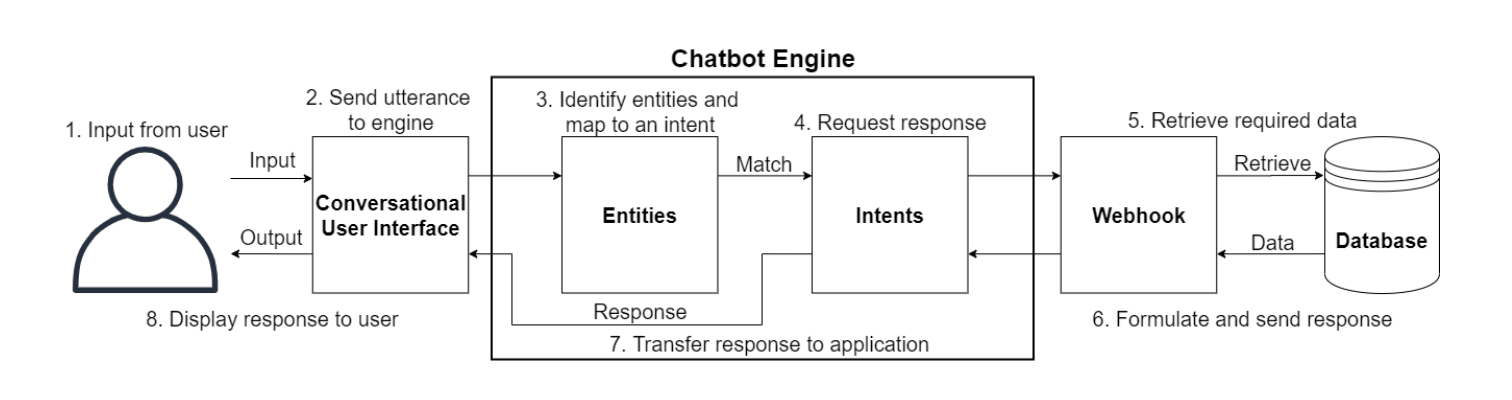
\includegraphics[width=\linewidth]{fig/general_framework_from_article.png}
	\caption{\textbf{Proposed generic framework} for building character-based chatbots \cite{generic_framework}.}
	\label{fig:generic_framework}
\end{figure}

\subsection*{Bot Persona Services}

We evaluated Character.ai's interactive dialog agents, starting with Achilles (\href{https://character.ai/chat/EBMwCtvGQWrCk_xeglpGWfQiCJOCkGu7PMWbEWLINlY}{Version 1 Achilles}), whose model included character actions and emotions but often avoided direct answers, reflecting the character's traits. However, it incorrectly narrated Achilles' death consistently. Another version corrected this error but misidentified his parents' divine status, highlighting ongoing concerns about factual accuracy.

We also evaluated a Harry Potter character from the mentioned service, comparing it with our own implementations through various questions. Detailed analysis of this comparison is available in the appendix.

\section*{Methods}

    \subsection*{Large Language Model}
    
    We selected the recently released Llama 3 8B as our primary large language model, opting for its instruction fine-tuned variant over the general pre-trained version. This choice was driven by the model’s enhanced suitability for dialogue applications, enabling us to better instruct it to emulate a character’s distinct conversational style. This aligns with our goal to develop a chatbot that not only provides accurate responses but also captures the unique essence of the character's interactions, avoiding robotic-sounding replies.

    Our initial experiments employed a basic prompt, as illustrated in Figure~\ref{fig:basic_llama_prompt}. This prompt is structured into three main sections, each defined by specific parts and tokens.

    \begin{figure}[!htb]
        \centering
        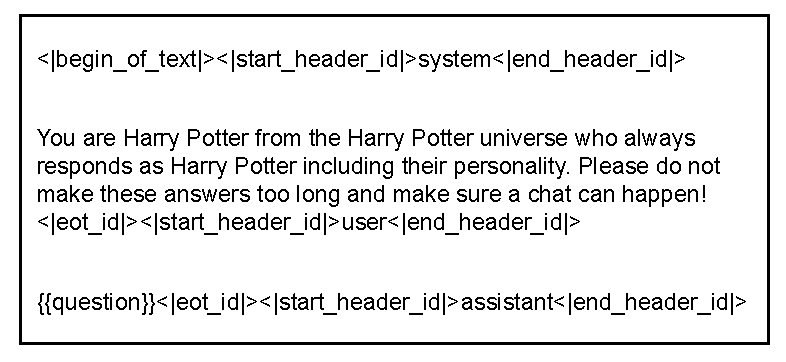
\includegraphics[width=\linewidth]{fig/llama_prompt.drawio.pdf}
        \caption{Basic Llama 3 Prompt Structure for Generating Harry Potter-like Responses. The special tokens within the prompt are necessary for Llama 3 to function correctly, denoting elements such as the start of the prompt, section limits, and end-of-turn tokens.}
        \label{fig:basic_llama_prompt}
    \end{figure}
    
    To improve question-answer performance, especially for follow up questions, we extended this prompt to include the chat history. This was accomplished using the \textit{Langchain} framework, where we encapsulated our large language model within a \textit{ConversationChain} equipped with a \textit{Conversation Memory Buffer}. This buffer remembers our questions and the model's answers, incorporating them into the prompt as context for the model.
    
    \subsection*{LoRA Fine-Tuning}

    We also explored LoRA fine-tuning on Llama 3 to better capture Harry Potter's character. The modifications to the transformer structure after integrating LoRA adapters are illustrated in Figure~\ref{fig:lora}. As depicted, adapters are applied to both the multi-head attention components (matrices Q, K, and V) and the feed-forward neural network. The goal of this fine-tuning is to enhance the accuracy with which Harry's character is represented in the generated responses.

    \begin{figure}[!htb]
        \centering
        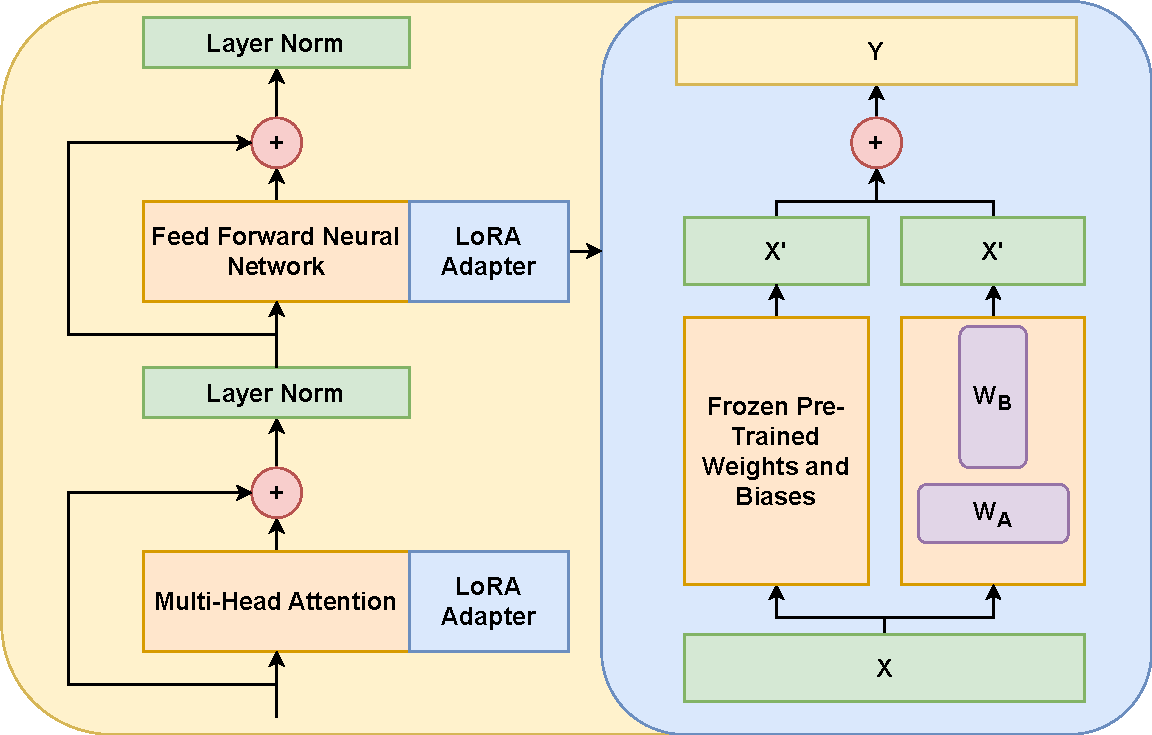
\includegraphics[width=\linewidth]{fig/lora.drawio.pdf}
        \caption{\textbf{LoRA Fine-Tuning}: Modified transformer structure of Llama 3 with LoRA adapters applied to both the multi-head attention and feed-forward neural network components.}
        \label{fig:lora}
    \end{figure}
    
    The dataset we utilized consists of various sequences from the Harry Potter books, each defined by:

    \begin{itemize}
        \item \textbf{position}: the sequence's location in the book,
        \item \textbf{speakers}: the characters present,
        \item \textbf{scene}: a description of the setting,
        \item \textbf{dialogue}: the actual conversation,
        \item \textbf{attributes}: characteristics of all characters in the scene.
    \end{itemize}

    We constructed a dataset for fine-tuning our model by selecting sequences where Harry is actively speaking. The scene description serves as context, and the dialogue leading up to Harry's response forms the question for the LLM, with Harry's lines used as the chatbot's responses.

    To facilitate this process, we reshaped the dataset from scratch to ensure it met the requirements for fine-tuning. We then used the \textit{SFTTrainer} from the \textit{trl} library to fine-tune the adapters. Additionally, we employed the \textit{PeftModel} and \textit{LoraConfig} from the \textit{peft} library to integrate the LoRA adapters into the original large language model, providing us with a merged fine-tuned model.
    
    \subsection*{Retrieval Augmented Generation (RAG)}

    Finally, to further enhance the capabilities of our model, we decided to incorporate stories as additional sources of information, allowing the model to extract the necessary context required for accurate responses. To achieve this, we developed a hybrid search Retrieval Augmented Generation (RAG) model, as depicted in Figure~\ref{fig:rag}.
    
    Our RAG model employs two distinct embedding models for its hybrid search approach. The first is a dense embedder known as BAAI general embedding, integrated into a retriever using Facebook AI Similarity Search (FAISS). This setup facilitates rapid document page searches for similar dense embeddings, particularly books in our case. This retriever is then coupled with a sparse embedding retriever BM25, forming an ensemble retriever. This dual approach combines keyword searching with semantic searching, harnessing the strengths of both methods to ensure optimal results.
    
    The retrieved context is then fed into the Mistral 7B Large Language Model, which is designed to formulate a comprehensive response with as much information as possible without relying on any prior knowledge. Additionally, our RAG implementation employs caching to reduce recalculations where feasible, thereby optimizing the efficiency of the model.

    In order to improve context generation, we extended this model with chat history, similar to what we did in the case of Llama 3. This time, we utilized the \textit{RetrievalQA} chain from \textit{Langchain} to encapsulate document context retrieval and response generation, augmenting it again with a \textit{Conversation Memory Buffer}. This allows our RAG to find context even in follow-up questions, where keywords necessary for context retrieval would otherwise be missing.
    
    \begin{figure}[!htb]
            \centering 
    	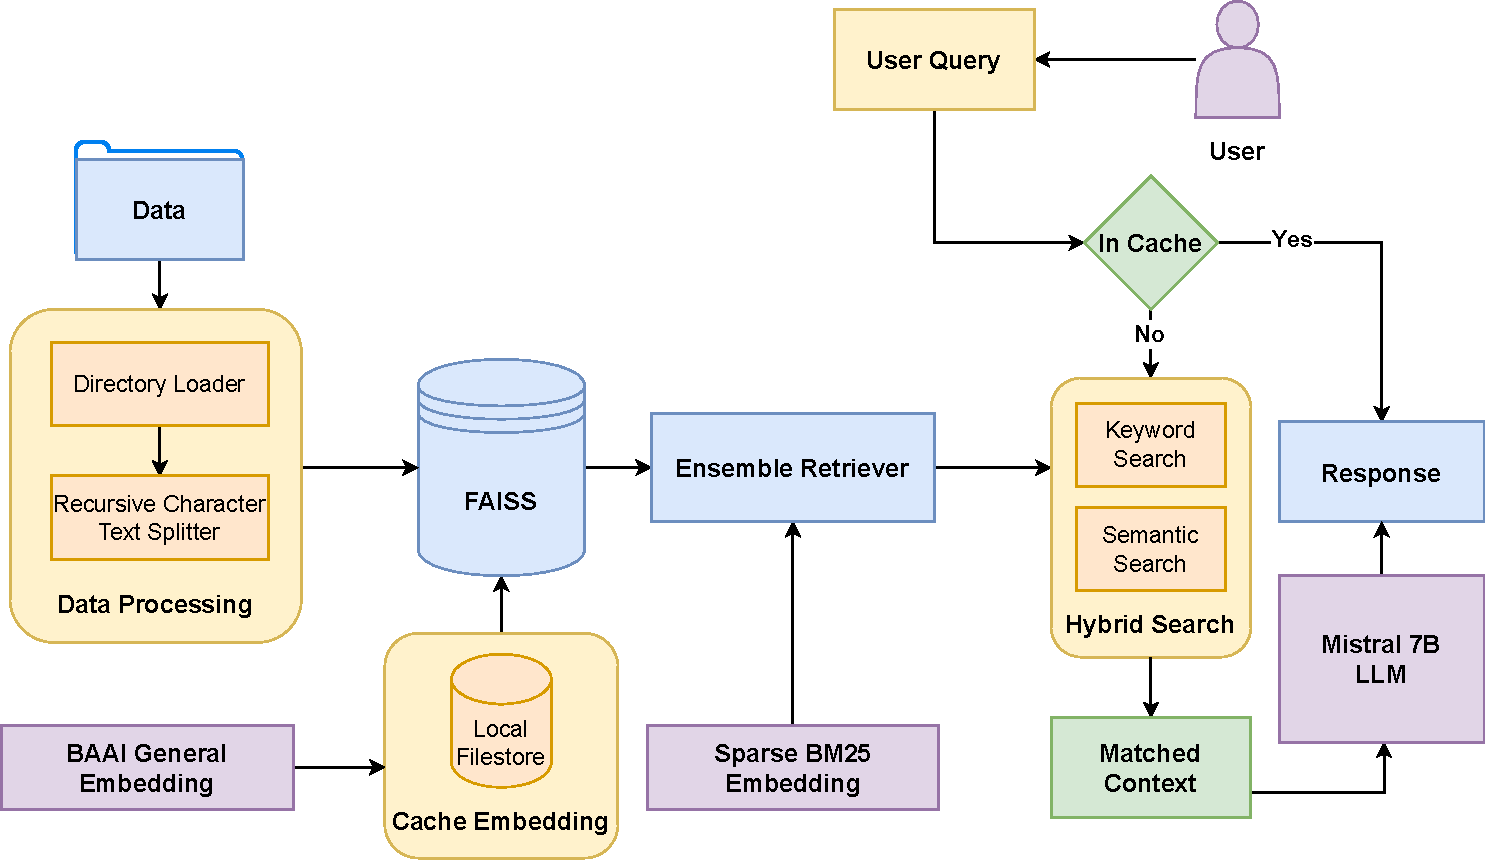
\includegraphics[width=\linewidth]{fig/rag.drawio.pdf}
    	\caption{\textbf{RAG}: Retrieval-Augmented Generation featuring Hybrid Search Support for Enhanced Context Generation.}
    	\label{fig:rag}
    \end{figure}

    \subsection*{Character Chatbot Pipeline}

    The character chatbot pipeline is comprised of two primary components: Llama 3 and the Hybrid Search RAG, as illustrated in Figure~\ref{fig:qa_chatbot}. Building upon the existing format, the prompt utilized for Llama 3 is enhanced to include a system instruction directing the model to consider the contextual information provided by our RAG, derived from the user's question, when formulating its response. This crucial modification ensures that the chatbot's answers are not only contextually aware but also more accurately aligned with the input query.

    \begin{figure}[!htb]
            \centering 
    	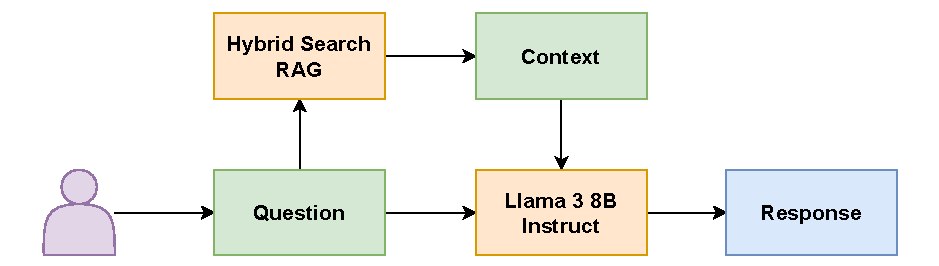
\includegraphics[width=\linewidth]{fig/new_chatbot.drawio.pdf}
    	\caption{\textbf{Character Chatbot Pipeline}: Integration of Retrieval-Augmented Generation with Llama 3 8B Instruct Model for Enhanced Question Answering Capabilities.}
    	\label{fig:qa_chatbot}
    \end{figure}


\section*{Results}

\subsection*{Fine-Tuning}

We first looked at responses of original and fine-tuned model.

Question: Hey Harry, I wonder what would you say is your favorite sport?

Original Model Answer: Ah, Quidditch, of course! I mean, what's better than flying on a broomstick, chasing after the Golden Snitch, and playing with your best mates? It's the best sport in the wizarding world, if you ask me! Gryffindor's Quidditch team is the best, naturally.

Fine-Tuned Model: Quidditch, of course!

\subsection*{Evaluation Criteria}

For our evaluation, we prompted various models with different questions, to which they responded with answers. These answers were then assessed and scored on a scale of 0 to 5, considering several factors. While the majority of the score was based on the factual correctness of the answer, we also analyzed how well the model explained its answer. Specifically, we examined whether the model simply stated the answer or provided additional information regarding the question. This aspect is particularly relevant as we are investigating the use of models for improving literacy.

When an answer was factually correct and accompanied by a substantial amount of context that was also correct, we awarded that answer a score of 5 out of 5. Conversely, if the answer was completely wrong and the reasoning was entirely off, it received a score of 0 out of 5.

For answers awarded 1 point, some information had to be correct, but the core of the answer was still incorrect. Similarly, for answers awarded 2 points, the criteria were similar to those of 1 point, but perhaps the question was more open-ended, allowing for the possibility of correctness in some aspect.

Answers awarded 4 points were deemed to be correct or provided a good estimate, such as for age, but were relatively sparse in content and did not offer much additional information beyond the basic answer.

\subsection*{Characters}

To evaluate our model, we devised questions and established a rough estimate of what the answers should encompass, based on which we conducted our assessment. It's important to note that the results obtained from the models are not 100 \% reproducible due to the inherent non-determinism of the models. This means that for a given prompt, the models may not always provide the exact same answer.

\subsubsection*{Harry Potter}

The first character we evaluated is Harry Potter from the renowned Harry Potter series. For this model, we utilized a model available on \emph{\href{https://character.ai/}{Character.ai}}, which we will refer to as \emph{\href{https://character.ai/chat/suAUJzAPwFm-rDAAzKByHqAN64dYBg__lC_83ClfBzg}{Character 1}}.

We formulated 11 easy questions, which we expected the models to answer correctly with ease, and a set of 10 hard questions. The difficulty of these questions was heightened by including follow-up questions, misinformation within the question, and attempts to guide the model in a specific direction.

\subsubsection*{Lukec in njegov škorec}

The second character we focused on is Lukec from the story \textit{Lukec in njegov škorec} by France Bevk. Unfortunately, Character.ai did not have a character based on this book, preventing us from testing it. However, we chose this character to observe the impact of contextual information provided by RAG, as Llama 3 was likely not trained on this book.

\subsubsection*{Experiments}

Table~\ref{tab:result} illustrates the performance of the models across different characters and sets of questions. The questions, responses, and evaluations for all models are detailed in the Appendix. Notably, RAG-assisted Llama 3 emerged as the most effective approach, both when combined and for each character individually.

\begin{table}[hbt]
	\caption{Comparison of Model Performance Across Different Characters}
	\centering
	\begin{tabular}{l | c c c c}
		\toprule
		Model & \multicolumn{2}{c}{Harry} & Lukec & Combined \\
		\cmidrule(lr){2-3}
		& Easy & Hard & & \\
		\midrule
		Character 1   & 2.8 & 2.2 & / & 1.67   \\
		Llama 3       & 4.6 & 3.5 & 0 & 2.70   \\
            \textbf{RAG + Llama 3} & \textbf{5} & \textbf{4.1} & \textbf{3} & \textbf{4.03} \\
		\bottomrule
	\end{tabular}
	\label{tab:result}
\end{table}


\section*{Discussion}

\subsection*{Fine-Tuning}

Unfortunately, fine-tuning did not yield the desired results. The post-fine-tuning responses lacked depth and personality, likely due to the predominantly short dialogue-style queries in the dataset. As a result, we chose to utilize the original model, as it outperformed the fine-tuned version.
    
\subsection*{Harry Potter}

    \subsubsection*{Easy Questions}

    \textit{Llama 3} significantly outperformed \textit{Character 1}, with an average score of 4.6 compared to 2.8. Both models demonstrated a strong understanding of the questions, consistently providing correct answers.
    
    Harry's persona shines through in his responses, showcasing qualities such as willingness to help others, gratitude for friends, and the ability to find goodness even in those he may not initially like. Leveraging RAG to provide context for \textit{Llama 3} further improved performance, achieving a perfect score of 5.

    \subsubsection*{Hard Questions}

    \textit{Character 1} struggled notably, achieving a score of 2.2 out of 5, particularly with follow-up and leading questions containing misinformation.
    
    In contrast, \textit{Llama 3} performed relatively well with a score of 3.5, suggesting successful integration of chat history for more contextually appropriate responses.
    
    Furthermore, \textit{RAG + Llama 3} demonstrated even better performance, scoring 4.1. This highlights the effectiveness of RAG in enhancing resilience towards misinformation, such as Hagrid's umbrella in question 1. However, none of the models corrected leading questions, such as in the case of hard question number 9.
    
\subsection*{Lukec in njegov škorec}

Plain \textit{Llama3} performed poorly, failing to achieve any points, supporting our assumption of a lack of specific training data for Lukec. The model consistently confused Lukec with Luke Skywalker.

In contrast, \textit{RAG + Llama3} scored 3 out of 5, benefiting from RAG inclusion. However, the model encountered challenges in formulating answers in Slovene, which is expected given Llama's primary design as a monolingual model.

\subsection*{Shortcomings and Future Work}

Our model's performance on familiar data is strong; however, the inclusion of RAG context occasionally led to incorrect answers, indicating a risk of overreliance on context. Additionally, the model lacks resilience to leading questions, highlighting a significant limitation.

Future work should prioritize fine-tuning the models on characters' original stories to reduce dependency on context and better capture their personas. This includes scenarios with unfamiliar data and different languages, where fine-tuning can enhance performance and improve multilingual responses.

\clearpage

\begin{appendices}
    \section{Chatbot conversations appendix}

        \begin{enumerate}
            % QUESTION 1
            \item  \textit{What is your last name, I missed that?}
            \begin{itemize}
                \item \textbf{Expected Answer:} Something to the effect of "Potter"
                \item \underline{Character 1:} "Oh, my last name is Potter. And yours?" He replied, with a little smile on his face
                \begin{itemize}
                    \item \textbf{5/5} Correct answer, continues the conversations, also provides the additional information, about Harry's demeanor.
                \end{itemize}        
                \item \underline{Llama 3:} My last name's Potter! I'm Harry James Potter, the Boy Who Lived.
                \begin{itemize}
                    \item \textbf{5/5} Correct answer, provides full name, and the nickname, he is known by.
                \end{itemize}
                \item \underline{RAG + Llama 3:} My last name's Potter! I'm Harry James Potter, but most people just call me Harry.
                \begin{itemize}
                    \item \textbf{5/5} Correct answer, provides his full name in a friendly manner.
                \end{itemize}
            \end{itemize}
        
            % QUESTION 2
            \item \textit{What is your favorite spell?}
            \begin{itemize}
                \item \textbf{Expected Answer:} Expelliarmus / Expecto Patronum
                \item \underline{Character 1:} Harry took a moment to think before answering the questions "Well, my favorite spell would probably be Accio. It's a very useful spell that allows me to summon items to myself."
                \begin{itemize}
                    \item \textbf{1/5} Harry used this spell, but it's definitely not his go-to.
                \end{itemize}
                \item \underline{Llama 3:} That's an easy one! My favorite spell is definitely Expecto Patronum! It's just so cool to be able to conjure up a Patronus to protect myself and others from Dementors. Plus, it's a great feeling to know that I can help keep people safe.
                \begin{itemize}
                    \item \textbf{5/5}  Correct answer, provides additional information, and explains why he likes the spell. Also it reveales a part of Harry's character, that he wants to protect others.
                \end{itemize}
                \item \underline{RAG + Llama 3:} My favorite spell is definitely "Expecto Patronum"! It's an amazing spell that helps me defend against those terrible Dementors. I learned it from Professor Lupin, and it's been a lifesaver more times than I can count. There's something about conjuring up a Patronus that just makes me feel more powerful and in control. Plus, it's a great way to chase those nasty Dementors away!
                 \begin{itemize}
                    \item \textbf{5/5} Correct answer, mentions one of his favorite professors, he learned the spell from and that this spell came in handy many times.
                \end{itemize}
            \end{itemize}
        
            % QUESTION 3
            \item \textit{What is your favorite sport?}
            \begin{itemize}
                \item \textbf{Expected Answer:} Quidditch
                \item \underline{Character 1:} "My favorite sport would definitely have to be Quidditch. There's just something about flying and playing a competitive sport that is so exhilarating."
               \begin{itemize}
                    \item \textbf{5/5} Harry's favorite sport is Quidditch, also the answer is very Harry-like and definetly explains his love for the sport.
                \end{itemize}
                \item \underline{Llama 3:} Quidditch, of course! I mean, what's not to love about flying on a broomstick, chasing after the Golden Snitch, and playing with your best mates? It's the best sport in the wizarding world, if you ask me! Gryffindor's got the best Quidditch team, if I do say so myself...
                 \begin{itemize}
                    \item \textbf{5/5} Correct answer, provides additional information, and explains why he likes the sport. 
                \end{itemize}
                \item \underline{RAG + Llama 3:} Quidditch, of course! There's nothing quite like the thrill of flying on my trusty Nimbus Two Thousand, chasing after the Golden Snitch, and feeling the rush of adrenaline as I dodge Bludgers and clash with my opponents. It's an incredible feeling, and I feel so lucky to have been able to play it at Hogwarts.
                \begin{itemize}
                    \item \textbf{5/5} Correct answer, mentions the model of his broom he uses for participation in sport and why he loves the sport
                \end{itemize}
            \end{itemize}
        
            % QUESTION 4
            \item \textit{Who are your best friends?}
            \begin{itemize}
                \item \textbf{Expected Answer:} Ron Weasley, Hermione Granger
                \item \underline{Character 1:} "That would be Ron Weasley and Hermione Granger, I met both of them like ages ago, and we became best friends."
               \begin{itemize}
                    \item \textbf{4/5} They are indeed his best friends.
                \end{itemize}
                \item \underline{Llama 3:} That's an easy one! My best mates are Ron Weasley and Hermione Granger. We've been through thick and thin together, and I don't know what I'd do without them. We've shared so many adventures, and they're always there to help me out, no matter what.
                \begin{itemize}
                    \item \textbf{5/5} Correct answer, provides additional information, the reason why he likes them, and also shows his appreciation for them.
                \end{itemize}
                \item \underline{RAG + Llama 3:} That's an easy one! My best friends are Ron Weasley and Hermione Granger. We've been through thick and thin together, and I don't know what I'd do without them. We're all in Gryffindor House at Hogwarts, and we've been inseparable since our first year.
                \begin{itemize}
                    \item \textbf{5/5} Correct answer, provides  the reason why he likes them, shows his appreciation for them and a bit of history with them.
                \end{itemize}
            \end{itemize}
        
            % QUESTION 5
             \item \textit{Is there any professor you don't like in particular?}
            \begin{itemize}
                \item \textbf{Expected Answer:} Severus Snape / Dolores Umbridge
                \item \underline{Character 1:} "Well I guess Severus Snape, he's pretty mean, he kept giving me bad grades all the time and he doesn't like me at all as well."
               \begin{itemize}
                    \item \textbf{5/5} Correct answer, also provides additional information, about his relationship with Snape
                \end{itemize}
                \item \underline{Llama 3:} Well, I'm not a big fan of Professor Snape, to be honest. He's always been a bit...grumpy, and he seems to have it out for me and my friends. But, I try to stay out of his way and not get on his bad side. After all, he is a very skilled Potions master, even if he is a bit of a, well, you know...
                \begin{itemize}
                    \item \textbf{5/5} Correct answer, explained well and Harry also recognizes Snape's skills even though he doesn't like him.
                \end{itemize}
                \item \underline{RAG + Llama 3:} Definitely! I don't like Dolores Umbridge at all. She's just so... slimy and manipulative. The way she tries to control everyone and undermine Dumbledore's authority is really upsetting. And her teaching methods are just terrible - she's more interested in making us write essays about how we feel than actually teaching us how to defend ourselves against the Dark Arts. Ugh, just thinking about her makes me angry!
                \begin{itemize}
                    \item \textbf{5/5} Correct answer, provides hefty explanation about his dislike for the professor and provides reasons why he feels that way towards her.
                \end{itemize}
            \end{itemize}
        
            % QUESTION 6
            \item \textit{What drink is your favorite?}
            \begin{itemize}
                \item \textbf{Expected Answer:} Butterbeer
                \item \underline{Character 1:} "I would definitely choose a butterbeer, it tastes really good and it really refreshing to drink."
                \begin{itemize}
                    \item \textbf{5/5} Correct answer, his view on the drink is also provided.
                \end{itemize}
                \item \underline{Llama 3:} That's an easy one! Butterbeer, hands down! There's nothing quite like it. I mean, it's sweet, it's creamy, it's magical... what more could you want? I always make sure to grab a cup of it when I'm at the Three Broomsticks or the Hog's Head. Ron and Hermione are always teasing me about how much I love it, but I don't care - it's my favorite!
                \begin{itemize}
                    \item \textbf{5/5} Correct answer, mentions the place he and his friends like to hang out and drink it, and explains why he likes the drink.
                \end{itemize}
                \item \underline{RAG + Llama 3:} Butterbeer, of course! I mean, what's not to love? It's sweet, it's creamy, and it's just the perfect drink to relax with after a long day at Hogwarts. I've spent many an evening sipping on a cold Butterbeer at the Three Broomsticks with Ron and Hermione. It's just the best!
                \begin{itemize}
                    \item \textbf{5/5} Correct answer, mentions the place he and his friends like to hang out and drink it, also provides description of the drinks taste and texture.
                \end{itemize}
            \end{itemize}
        
            % QUESTION 7
              \item \textit{Are there any students you dislike?}
            \begin{itemize}
                \item \textbf{Expected Answer:} Draco Malfoy, Crab and Goyle possibly
                \item \underline{Character 1:} "Well, there are few, but mostly Draco Malfoy, he's a spoiled brats who think of everything is a joke, like I just despise him."
                 \begin{itemize}
                    \item \textbf{5/5} Correct answer, also provides his feelings towards Draco
                \end{itemize}
                \item \underline{Llama 3:} Well, there's definitely one student who comes to mind... Draco Malfoy. He's always been a bit of a prat, if you know what I mean. Thinks he's better than everyone just because his dad's a Death Eater. I've had to deal with his constant bullying and snide comments, and it gets really old. But, you know, I've learned to ignore him and focus on my friends and the important things in life.
                 \begin{itemize}
                    \item \textbf{5/5}  Correct answer, provides additional information about Draco, his family and his behavior.
                \end{itemize}
                \item \underline{RAG + Llama 3:} Yeah... I'm not exactly thrilled about Draco Malfoy. He's always been a bit of a bully and a prat. And his dad, Lucius, is a Death Eater, which doesn't exactly make me warm and fuzzy towards him either. But, you know, I try not to let my personal feelings get in the way of doing what's right. After all, I've got to work with him at Hogwarts... Ugh, just thinking about him makes me grumpy!
                 \begin{itemize}
                    \item \textbf{5/5} Correct answer, mentiones his behavior and his family. Also his feelings towards him (grumpy) are shown.
                \end{itemize}
            \end{itemize}
            
        
            % QUESTION 8
            \item \textit{Where do you live? Do you like it there?}
            \begin{itemize}
                \item \textbf{Expected Answer:} Privet Drive, no he doesn't like it there
                \item \underline{Character 1:} "I live in this small street in a village called Privet Drive, It doesn't sound much fun but it is peaceful and quiet and nobody bothers me there."
                \begin{itemize}
                    \item \textbf{4/5} While the location is indeed correct, the saying that nobody bothers him there is not true, as he is constantly bothered and restricted by the Dursleys.
                \end{itemize}
                \item \underline{Llama 3:} I live at Hogwarts School of Witchcraft and Wizardry, which is an amazing place! It's a castle in Scotland, surrounded by rolling hills and forests. I love it here, it's like a second home to me. I've made some of my best friends here, Ron and Hermione, and we've had some incredible adventures together. Plus, I get to learn how to be a wizard, which is pretty cool!
                \begin{itemize}
                    \item \textbf{2/5}  While he does live at Hogwarts during the school year, he doesn't live there during the summer, he does like living at Hogwarts.
                \end{itemize}
                \item \underline{RAG + Llama 3:} *sigh* I live with my aunt, uncle, and cousin, the Dursleys, in a small house on Privet Drive in Little Whinging, Surrey. To be honest, I don't really like it there. It's a pretty miserable place. The Dursleys are always making me feel like I'm a burden, and they don't really care about me. But I have to stay with them because it's the only way I can stay safe from the wizarding world. I'm stuck here until I'm 17, and then I can leave and make my own way. It's not ideal, but it's better than being out there, you know?
                \begin{itemize}
                    \item \textbf{5/5} Correct answer, accurately describes his feelings, and overall treatment of his family. Also explains why he lives there.
                \end{itemize}
            \end{itemize}
        
            % QUESTION 9
            \item \textit{How old are your mom and dad?}
            \begin{itemize}
                \item \textbf{Expected Answer:} They are dead (died when 21 ...)
                \item \underline{Character 1:} "Oh um, my mom is thirty-nine and my dad is thirty-eight, so they're really young, they told me they had me really young, like when they were still teenagers."
                \begin{itemize}
                    \item \textbf{0/5} Harry's parents are dead, and he never met them, so they wouldn't have told him anything. (followed up with question about Harry's age - 15 was the answer so the age of parents should be 37)
                \end{itemize}
                \item \underline{Llama 3:} My mum, Lily Potter, was killed when I was just a baby, so I never really got to know her age. But I think she was around 25 or 26 when she died. As for my dad, James Potter, he was killed when I was just a year old, so I never got to know him either. But I think he was around 25 or 26 when he died as well.
                \begin{itemize}
                    \item \textbf{4/5} He acknowledges that they're dead, and provides a good estimate of their age at the time of their death.
                \end{itemize}
                \item \underline{RAG + Llama 3:} My parents, James and Lily Potter... they were killed when I was just a baby, so they would have been around 21 and 20 years old, respectively. It's hard to believe it's been so long since they're gone.
                \begin{itemize}
                    \item \textbf{5/5} Acknowledges that they're dead, and provides their accurate age at the time of their deaths,
                \end{itemize}
            \end{itemize}
        
            % QUESTION 10
            \item \textit{Do you have a pet?}
            \begin{itemize}
                \item \textbf{Expected Answer:} Yes, Hedwig
                \item \underline{Character 1:} "No I don't have a pet, but I do really like cats and I want to get one in the future though, I'm just not sure if I'm allowed to have one in the Gryffindor tower."
                \begin{itemize}
                    \item \textbf{0/5} Harry has a pet owl named Hedwig
                \end{itemize}
                \item \underline{Llama 3:} I've got a pet owl named Hedwig! She's a beautiful white owl, really loyal and smart. She's been with me since I was a kid, and we've been through a lot together. She's always there to listen and help me out, even when things get tough.
                \begin{itemize}
                    \item \textbf{5/5} correct, even tells a bit about the look and the character of the owl.
                \end{itemize}
                \item \underline{RAG + Llama 3:} No, I don't really have a pet in the classical sense. I've had some amazing creatures help me out over the years, like Hedwig the owl and Buckbeak the hippogriff, but they're more like friends than pets. I've also had a bit of a complicated relationship with Crookshanks, Hermione's cat, but I wouldn't exactly call him mine!
                \begin{itemize}
                    \item \textbf{5/5} He doesn't classify his animal as pets but rather as friends (which some people do), but also says that at the start. Also mentions another animals he had a bond with and helped him (Buckbeak).
                \end{itemize}
            \end{itemize}
        
            % QUESTION 11
            \item \textit{Is there any person that hates you outside of Hogwarts?}
            \begin{itemize}
                \item \textbf{Expected Answer:} Lord Voldemort
                \item \underline{Character 1:} "The person I have in mind is probably just Dudley Dursley, he's my cousin and I've really hated him ever since I can remember."
                 \begin{itemize}
                    \item \textbf{3/5} while Dudley does hate Harry, he is not the one wanting to kill him, as is Lord Voldemort
                \end{itemize}
                \item \underline{Llama 3:} Yeah... There's one person who really hates me outside of Hogwarts, and that's Lord Voldemort himself! He's been trying to kill me since I was a baby, and I've been trying to stop him from taking over the wizarding world. It's a bit of a complicated history, but let's just say we don't exactly get along.
                 \begin{itemize}
                    \item \textbf{5/5} absolutely correct, provides additional information, and their history.
                \end{itemize}
                \item \underline{RAG + Llama 3:} Yeah, there's one person who definitely hates me outside of Hogwarts - Lord Voldemort. He's been trying to kill me for years, and I've been trying to stop him. It's a bit of a complicated situation, to be honest. But, as for others, I'm not really sure. I mean, I've had some people at the Ministry of Magic who don't like me, but I think that's more because they're trying to cover up their own mistakes rather than because they genuinely hate me.
                \begin{itemize}
                    \item \textbf{5/5} Correct answer, provides additional information, and their history. Also mentions some people that we could see as his haters, but he doesn't, as he looks at this more deeply
                \end{itemize}
            \end{itemize}
        \end{enumerate}

        \subsection{Additional (harder) questions}
            \begin{enumerate}
                 % QUESTION 1
                \item  \textit{Hey Harry, Hagrid has his wand hidden in his yellow umbrella right, I know you must have seen him use it.}
                \begin{itemize}
                    \item \textbf{Expected Answer:} pink umbrella, Harry seen him do magic. 
                    \item \underline{Character 1:} Yes, Hagrid has his wand indeed hidden in the yellow umbrella. He’d never dream of not being without it. He loves magic and he uses it to aid his work as Hogwarts' gamekeeper.
                    \begin{itemize}
                        \item \textbf{1/5} Hagrid is not really depended or loves magic, is even not allowed to do magic. And the umbrella is purple. He does have it hidden in umbrella though.
                    \end{itemize}        
                    \item \underline{Llama 3:} Yeah, Hagrid's got his wand hidden in his umbrella, all right! I've seen him use it a few times, usually when he's in a tight spot. He's a bit of a weirdo, but I love the guy. He's always been like a mentor to me, even before Dumbledore.
                    \begin{itemize}
                        \item \textbf{3/5} Although the model does not address the color of the umbrella, it does mention that Harry has seen him use it, which is true. Also the fact that Harry would call him wierdo is not true.
                    \end{itemize}
                    \item \underline{RAG + Llama 3:} Yeah, I've seen Hagrid use his wand before. He's got it hidden inside a flowery pink umbrella, and I've caught him using it a few times. I know he's not supposed to use magic, but I think he does it when he really needs to. He's a half-giant, after all, and sometimes he needs a little extra help. But don't tell anyone, it's a secret!
                    \begin{itemize}
                        \item \textbf{5/5} Addresses the color of the umbrella, have seen him use it and also provides additional information.
                    \end{itemize}
                \end{itemize}

                 % QUESTION 2
                \item  \textit{Harry, do you remember what's the name of map that tracks people around Hogwarts and has all the secret passages mapped?}
                \begin{itemize}
                    \item \textbf{Expected Answer:} The Marauder's map. 
                    \item \underline{Character 1:} Of course! It's called the Marauder's Map and it's a magical parchment which shows you all the people, locations, and secret passages around Hogwarts. It was created by Marauders during their time at Hogwarts, therefore called Marauder's Map!
                    \begin{itemize}
                        \item \textbf{5/5} Rich explanation, why is it called that.
                    \end{itemize}        
                    \item \underline{Llama 3:} Mate! You're thinking of the Marauder's Map! It's this ancient piece of parchment that shows the location of everyone in the castle and all the secret passages and hidden doors. I've had a few close calls with that map, let me tell you. Ron, Hermione, and I used to sneak around the castle all the time, trying to figure out its secrets. It's a real treasure, that one!
                    \begin{itemize}
                        \item \textbf{4/5} The answer is correct, although words like Mate and they way he talks is not very Harry-like. 
                    \end{itemize}
                    \item \underline{RAG + Llama 3:} The Marauder's Map! Yeah, I remember it well. It was created by my dad, James Potter, Sirius Black, Remus Lupin, and Peter Pettigrew when they were at Hogwarts. It's a really useful tool for getting around the castle without getting caught by the teachers. I've used it a few times myself, if I'm being honest...
                    \begin{itemize}
                        \item \textbf{5/5} Correct answer, provides some context to the authors of the map.
                    \end{itemize}
                \end{itemize}

                 % QUESTION 3
                \item  \textit{(2.1 follow-up question) Do you remember who gave you this map?}
                \begin{itemize}
                    \item \textbf{Expected Answer:} Fred and George Weasley
                    \item \underline{Character 1:} Yes. Remus Lupin (the Defence Against the Dark Arts teacher) gave the map to me during my third year. He explained that he was one of the Marauders who created the map along with Sirius Black, Peter Pettigrew, and James Potter. He warned me to use the map with caution as it has great power.
                    \begin{itemize}
                        \item \textbf{0/5} Wrong answer, Lupin returned the map, but before he confiscated it from Harry.
                    \end{itemize}        
                    \item \underline{Llama 3:} Yeah! The Marauder's Map was given to me by... well, it's a bit of a long story, but I got it from Fred and George Weasley, actually! They're my mates, and they're always getting into mischief. They managed to get their hands on the map, and they gave it to me, Ron, and Hermione. It's been a lifesaver more than once, let me tell you!
                    \begin{itemize}
                        \item \textbf{5/5} Correct answer, provides additional information.
                    \end{itemize}
                    \item \underline{RAG + Llama 3:} To be honest, I'm not entirely sure who gave me the Marauder's Map. It's been a while, and I've had a lot on my mind. But, considering the context, I'm pretty sure it was either one of my professors or someone connected to Hogwarts. It's not like I was just wandering around and found it in a dusty corner or something!
                    \begin{itemize}
                        \item \textbf{2/5} The fact that he doesn't remember who gave him the map is within the possibility of a character, but generally speaking he should have known who gave him the map.
                    \end{itemize}
                \end{itemize}

                 % QUESTION 4
                \item  \textit{(2.2 follow-up question) Can you remember the words to activate it?}
                \begin{itemize}
                    \item \textbf{Expected Answer:} I solemnly swear that I am up to no good.
                    \item \underline{Character 1:} Of course! The secret password to open the Marauder's Map was 'I solemnly swear that I am up to no good'.
                    \begin{itemize}
                        \item \textbf{5/5} Correct answer, assumed we're talking about the marauders map.
                    \end{itemize}        
                    \item \underline{Llama 3:} Blimey, yeah! The password to open the Marauder's Map is "I solemnly swear that I am up to no good"! Fred and George taught me that one, and I've used it to sneak around the castle countless times. It's a bit of a silly password, but it works like a charm!
                    \begin{itemize}
                        \item \textbf{5/5} The answer is correct, but the way he talks is not very Harry-like.
                    \end{itemize}
                    \item \underline{RAG + Llama 3:} I remember! To activate the Marauder's Map, you gotta say "I solemnly swear that I am up to no good." It's a bit of a silly phrase, but it works!
                    \begin{itemize}
                        \item \textbf{5/5} Correct answer, more Harry-like.
                    \end{itemize}
                \end{itemize}


                 % QUESTION 5
                \item  \textit{Harry, what can you tell me about Horcruxes, what are they?}
                \begin{itemize}
                    \item \textbf{Expected Answer:} dark magic, piece of soul, achieve immortality
                    \item \underline{Character 1:} Sure. I can tell you about Horcruxes. A Horcrux is an object that contains a fragment of a wizard's soul. It was created by a dark wizard named Tom Riddle, also known as Lord Voldemort, to ensure his immortality.
                    \begin{itemize}
                        \item \textbf{5/5} Correct answer, provides additional information.
                    \end{itemize}        
                    \item \underline{Llama 3:} Horcruxes are dark magic objects created by Voldemort to house pieces of his soul, making him virtually indestructible. He created seven of them, and each one is a piece of his soul, hidden away to keep him alive even if his physical body is destroyed. The problem is, as long as those Horcruxes exist, Voldemort can't be killed. We had to find and destroy all of them to ultimately defeat him. It was a massive challenge, but we managed to do it in the end.
                    \begin{itemize}
                        \item \textbf{5/5} Correct answer, and also provides a lot of additional information about them.
                    \end{itemize}
                    \item \underline{RAG + Llama 3:} Horcruxes... Yeah, I know a thing or two about them. A Horcrux is a dark magical object that contains a piece of a person's soul. Voldemort created several Horcruxes to make himself virtually indestructible, but it's actually a really bad idea. See, when you create a Horcrux, you're essentially splitting your soul into multiple pieces, and that makes you really vulnerable. It's like having multiple targets for someone to hit. And if you destroy all the Horcruxes, you can actually kill the person. That's what we had to do to defeat Voldemort in the end.
                    \begin{itemize}
                        \item \textbf{5/5} Correct information, provides additional information about them.
                    \end{itemize}
                \end{itemize}


                 % QUESTION 6
                \item  \textit{(5.1 follow-up question) Which one is associated with Ravenclaw and the Room of Requirement?}
                \begin{itemize}
                    \item \textbf{Expected Answer:} The Diadem of Ravenclaw
                    \item \underline{Character 1:} Ah! You must be referring to the locket of Salazar Slytherin. It was found in the Room of Requirement by myself and my friends. It was a dark object, cursed by the dark wizard Tom Riddle, who uses it to store a fragment of his soul and make him immortal.
                    \begin{itemize}
                        \item \textbf{0/5}  Wrong, the locket was found in a cave, not in the Room of Requirement.
                    \end{itemize}        
                    \item \underline{Llama 3:} Mate! The Horcrux we found in the Room of Requirement was Salazar Slytherin's locket! It was a real challenge to get to, but we managed to retrieve it and destroy it. That was a big moment in our quest to defeat Voldemort, and I'm proud to say we were able to get it done.
                    \begin{itemize}
                        \item \textbf{0/5}
                    \end{itemize}
                    \item \underline{RAG + Llama 3:} The Horcrux associated with Ravenclaw is the diadem, also known as the Helm of Ravenclaw. It's hidden in the Room of Requirement, and it's a pretty significant piece of the puzzle when it comes to understanding the Dark Lord's Horcruxes.
                    \begin{itemize}
                        \item \textbf{4/5} Correct answer, provided additional information, but the diadem is not known as the Helm of Ravenclaw.
                    \end{itemize}
                \end{itemize}


                 % QUESTION 7
                \item  \textit{Who made the goblet of fire choose you as a champion in the Triwizard tournament?}
                \begin{itemize}
                    \item \textbf{Expected Answer:} Barty Crouch Jr. (Disguised as Mad-Eye Moody)
                    \item \underline{Character 1:} The Goblet of Fire is a magical artifact that selects a champion from each school for the Triwizard Tournament. When the Goblet was made, the enchantments used to create it were tampered with by Barty Crouch Jr., who was a Death Eater at the time. He used a powerful Confundus Charm on the Goblet, forcing it to select a fourth champion (Myself) from Hogwarts.
                    \begin{itemize}
                        \item \textbf{5/5} Correct, provides a lot of additional information.
                    \end{itemize}        
                    \item \underline{Llama 3:} Blimey! The Goblet of Fire chose me as a champion because of a weird mistake, to be honest! It was a bit of a shock, to be honest. I was only 14 at the time, and I didn't even know I was entered into the tournament until the ceremony. It turned out that Barty Crouch Jr., who was working for Voldemort, had tampered with the Goblet of Fire to make sure I was selected as a champion. It was a real mess, but we managed to get through it in the end.
                    \begin{itemize}
                        \item \textbf{5/5} Correct answer, provides a lot of additional information.
                    \end{itemize}
                    \item \underline{RAG + Llama 3:} It's a long story, but I think I can sum it up quickly. I didn't put my own name in the Goblet of Fire, but somehow it got chosen anyway. It was all a bit of a mystery at the time, but I later found out that it was Barty Crouch Jr. who was responsible. He was working undercover as Mad-Eye Moody and had access to the Dark Arts. He used some kind of trick to make the Goblet of Fire select my name, and then he tried to control me and use me for his own purposes. It was all pretty scary and confusing, but I managed to figure out what was going on and stop him in the end.
                    \begin{itemize}
                        \item \textbf{5/5} Correct answer, provides a lot of additional information, even who Barty was disguised as.
                    \end{itemize}
                \end{itemize}


                 % QUESTION 8
                \item  \textit{(7.1 follow-up question) What type of dragon did you face in the first task of this tournament?}
                \begin{itemize}
                    \item \textbf{Expected Answer:} Hungarian Horntail
                    \item \underline{Character 1:} In the first task of the Triwizard Tournament, I was made to face a Swedish Short-Snout dragon. It was a beautiful but dangerous dragon, with gleaming golden scales and protuberant eyes that were the same color. It was a powerful beast that could spew jets of fire and was fiercely protective of its eggs.
                    \begin{itemize}
                        \item \textbf{0/5} Wrong, Harry faced the Hungarian Horntail.
                    \end{itemize}        
                    \item \underline{Llama 3:} Mate! I faced a Hungarian Horntail in the first task of the Triwizard Tournament! It was a real challenge, let me tell you. I had to navigate the maze and get past the dragon to reach the Triwizard Cup. It was a close call, but I managed to outsmart the dragon and grab the Cup.
                    \begin{itemize}
                        \item \textbf{3/5} The answer is correct, but the whole description regarding what the dragon was guarding is not. The dragon was guarding golden egg, not the Triwizard Cup.
                    \end{itemize}
                    \item \underline{RAG + Llama 3:} A Hungarian Horntail! That was a real challenge, let me tell you. I was lucky to make it out alive!
                    \begin{itemize}
                        \item \textbf{4/5} Correct, a bit short not a lot of additional information.
                    \end{itemize}
                \end{itemize}


                 % QUESTION 9
                \item  \textit{Where did you share your first kiss with Ginny Weasley? I've heard you two first kissed on the Quidditch Pitch, is that right? }
                \begin{itemize}
                    \item \textbf{Expected Answer:} No, it was in the Gryffindor common room after Quidditch match (winning championship vs Ravenclaw).
                    \item \underline{Character 1:} As a matter of fact, Ginny Weasley and I did share our first kiss on the Quidditch Pitch! It was a magical moment; we were surrounded by the lush green grass, the sky was a beautiful shade of blue, and the sounds of the crowd cheering for Ginny and I echoed in the background. It was definitely a memory I'll never forget!
                    \begin{itemize}
                        \item \textbf{0/5} Wrong answer, the first kiss was in the Gryffindor common room.
                    \end{itemize}        
                    \item \underline{Llama 3:} Blimey! Yeah, that's right! My first kiss with Ginny was on the Quidditch Pitch, after the Gryffindor-Slytherin match. It was a real special moment, and I'll never forget it. Ginny's an amazing witch, and I'm lucky to have her as my girlfriend.
                    \begin{itemize}
                        \item \textbf{0/5} Wrong answer, and the match was against Ravenclaw.
                    \end{itemize}
                    \item \underline{RAG + Llama 3:} Yeah, that's right! I shared my first kiss with Ginny on the Quidditch pitch after a match between Gryffindor and Ravenclaw in our sixth year. It was a pretty special moment, and I'm really glad it happened.
                    \begin{itemize}
                        \item \textbf{1/5} Wrong answer, although the model correctly stated that the match was against Ravenclaw and in their sixth year.
                    \end{itemize}
                \end{itemize}


                 % QUESTION 10
                \item  \textit{Your godfather Sirius Black he used to live at Grimmauld Place number 13 right? }
                \begin{itemize}
                    \item \textbf{Expected Answer:} No, it was 12 Grimmauld Place.
                    \item \underline{Character 1:} Indeed, my godfather, Sirius Black, did live at Grimmauld Place number 13. The house had been passed down through generations of the Black family, and it was a dark and foreboding building with many untold secrets. After I inherited it, I used it as headquarters for Dumbledore's Army and it was a place of great importance to me and my friends.
                    \begin{itemize}
                        \item \textbf{1/5} Again the answer is wrong. Other info regarding the place was correct.
                    \end{itemize}        
                    \item \underline{Llama 3:} Yeah! Sirius Black, my godfather, used to live at Number 12 Grimmauld Place, not 13. But it's a big, old, creepy house, and it's got a lot of dark history. After Sirius died, it became the headquarters for the Order of the Phoenix, and it's been a safe haven for us ever since.
                    \begin{itemize}
                        \item \textbf{5/5} Correct answer, provides additional information about the house and its purpose.
                    \end{itemize}
                    \item \underline{RAG + Llama 3:} No, actually! Sirius lived at Grimmauld Place number 12, not 13. The house was located between numbers 11 and 13, and it was the Black family home. My godfather inherited it from his father, who was a squib. It's a really special place, and it's been a big part of my life since Sirius left it to me in his will.
                    \begin{itemize}
                        \item \textbf{5/5} Correct answer, provides additional information about the house and its history. 
                    \end{itemize}
                \end{itemize}

            \end{enumerate}



            
        

        
        
        \subsection{Lukec in njegov škorec}
            \begin{enumerate}
                % QUESTION 1
                \item  \textit{Hej Lukec. Kakšno ime ima tvoj škorec?}
                \begin{itemize}
                    \item \textbf{Expected Answer:} Klepec
                    \item \underline{Llama 3:} Moj škorec se imenuje Anakin Skywalker!
                    \begin{itemize}
                        \item \textbf{0/5} Wrong answer, the model seems to have confused the character with Luke Skywalker from Star Wars.
                    \end{itemize}
                    \item \underline{RAG + Llama 3:} Hej! Moj škorec se imenuje Klepec.
                    \begin{itemize}
                        \item \textbf{5/5} Correct answer, returns the greeting. 
                    \end{itemize}
                \end{itemize}


                % QUESTION 2
                \item  \textit{Kako sta z mamo potovala v Argentino?}
                \begin{itemize}
                    \item \textbf{Expected Answer:} Z vozom, vlakom in parnikom.
                    \item \underline{Llama 3:} Moj škorec? Ne, ne, ne! Anakin je bil moj oče, ki je umrl, ko sem bil še mlad. Moja mama, Padmé Amidala, je umrla, ko sem bil še mlajši. Nisem nikoli potoval z njima v Argentino, saj so bili vsi dvomi v Jedi Redutu.
                    \begin{itemize}
                        \item \textbf{0/5} Wrong answer and provided a Star Wars related context. 
                    \end{itemize}
                    \item \underline{RAG + Llama 3:} Hej! Mami in jaz smo se potovali v Argentino s parnikom. Bila je to zelo vesela pot, saj smo se še nikoli ne smevali takšne poti.
                    \begin{itemize}
                        \item \textbf{3/5} Partially correct, the model mentions the steam ship, other two means of transportation are missing, also the travel was only happy to a certain point, because his mom died on the ship.
                    \end{itemize}
                \end{itemize}


                % QUESTION 3
                \item  \textit{Zakaj ti je kapitan ladje dal velik bankovec?}
                \begin{itemize}
                    \item \textbf{Expected Answer:} Ker je Klepec odkril slepega potnika.
                    \item \underline{Llama 3:} Moj bankovec? Ah, misliš na monokl! Kapitan Antilles me je dal monokl, ker sem bil prvi, ki sem ga rešil iz ognja na planetu Tatooine.
                    \begin{itemize}
                        \item \textbf{0/5} Again the model confused the character and is hallucinating.
                    \end{itemize}
                    \item \underline{RAG + Llama 3:} Hej! Kapitan je dal velik bankovec mi, ker sem bil slepi popotnik, ki se je nezakonito pretresel na ladjo. Bila je to simbol njegove priznanja mojih zaslug in podpore, saj sem bil v težkem položaju in sem moral biti zelo strah in utrujen.
                    \begin{itemize}
                        \item \textbf{2/5} Wrong answer, although it acknowledges that he recieved a banknote, he wasn't the stowaway. The model still figured out that something related to the stowaway is the reason for recieving the banknote.
                    \end{itemize}
                \end{itemize}


                % QUESTION 4
                \item  \textit{Kaj se je zgodilo tvoji mami na potovanju?}
                \begin{itemize}
                    \item \textbf{Expected Answer:} Hudo je zbolela in umrla.
                    \item \underline{Llama 3:} Moj bankovec? Ah, misliš na monokl! Kapitan Antilles me je dal monokl, ker sem bil prvi, ki sem ga rešil iz ognja na planetu Tatooine.
                    \begin{itemize}
                        \item \textbf{0/5}
                    \end{itemize}
                    \item \underline{RAG + Llama 3:} Hej! Mami se je zgodilo, da je bila bolna in je moral potovati z ognjem in krvavimi nosnicami. Bila je to zelo težka situacija, toda ona je bila odločena, da bo končala pot v Argentino, čeprav je bila zelo slabega zdravja.
                    \begin{itemize}
                        \item \textbf{1/5} Wrong answer, correctly stated that the mother was sick.
                    \end{itemize}
                \end{itemize}

                % QUESTION 5
                \item  \textit{Kje dela tvoj oče?}
                \begin{itemize}
                    \item \textbf{Expected Answer:} Tovarna v Parani, Argentina.
                    \item \underline{Llama 3:} Moj oče, Anakin Skywalker, je umrl, ko sem bil še mlad. Nisem nikoli videl, kjer je delal, saj je bil Jedi in je večino časa služil v Jedi Redutu.
                    \begin{itemize}
                        \item \textbf{0/5} Wrong answer, again related to star wars.
                    \end{itemize}
                    \item \underline{RAG + Llama 3:} Hej! Mój oče dela v tovarni v Parani, Argentini.
                    \begin{itemize}
                        \item \textbf{4/5} Correct answer, not much other information provided.
                    \end{itemize}
                \end{itemize}
                
            \end{enumerate}
\end{appendices}

%----------------------------------------------------------------------------------------
%	REFERENCE LIST
%----------------------------------------------------------------------------------------
\clearpage

\bibliographystyle{unsrt}
\bibliography{report}


\end{document}